\documentclass[screen, aspectratio=169]{beamer}
\usepackage[T1]{fontenc}
\usepackage[utf8]{inputenc}
\usepackage{tikz, environ}
\usepackage{listings}
\usepackage{pgfplots}
\usepackage{arrayjob}
% Use the NTNU-temaet for beamer 
% \usetheme[style=ntnu|simple|vertical|horizontal, 
%     language=bm|nn|en, 
%     smalltitle, 
%     city=all|trondheim|alesund|gjovik]{ntnu2017}
\usetheme[style=horizontal,language=bm]{ntnu2017}

\usepackage[norsk]{babel}

\RequirePackage{listings, color, textcomp}
\lstset{
	tabsize=2,
	rulecolor=,
	basicstyle=\ttfamily\small,
	upquote=true,
	aboveskip={1.5\baselineskip},
	columns=fixed,
	showstringspaces=false,
	extendedchars=true,
	literate={æ}{{\ae}}1
			 {ø}{{{\o}}}1
			 {å}{{\aa}}1
			 {Æ}{{\AE}}1
			 {Ø}{{\O}}1
			 {Å}{{\AA}}1,
	breaklines=true,
	breakatwhitespace=true,
	escapeinside={(*}{*)},
	showtabs=false,
	showspaces=false,
	keepspaces=true,
	showstringspaces=false,
	frame=l,
	identifierstyle=\ttfamily,
	keywordstyle=\color[rgb]{1.0,0,0},
	keywordstyle=[1]\color[rgb]{0,0,0.75},
	%keywordstyle=[2]\color[rgb]{0.5,0.0,0.0},
	keywordstyle=[3]\color[rgb]{0.127,0.427,0.514},
	keywordstyle=[4]\color[rgb]{0.4,0.4,0.4},
	commentstyle=\color[rgb]{0.133,0.545,0.133},
	stringstyle=\color[rgb]{0.639,0.082,0.082},
	mathescape
}
\lstset{language=Python}

\setbeamertemplate{section in toc}{%
	--- \inserttocsection \par}
\setbeamertemplate{subsection in toc}{%
	\hskip2em $\bullet$ \hspace{3pt} \inserttocsubsection \par}

\title[Short title]{Øvingsforelesning 9 i Python (TDT4110/TDT4127)}
\subtitle{Repetisjon}
\author[O.M. Pedersen]{Ole-Magnus Pedersen}
\institute[NTNU]{}
\date{}
%\date{} % To have an empty date

\hypersetup{colorlinks,
	urlcolor={blue!70!black},
	linkcolor=black
}

\AtBeginSection{
	\begin{frame}{Oversikt}
		\tableofcontents[currentsection]
	\end{frame}
}

\usetikzlibrary{decorations, positioning, calc}

\begin{document}

\begin{frame}
  \titlepage
\end{frame}

\section{Praktisk Informasjon}
\begin{frame}{Praktisk Informasjon}
    \begin{itemize}
        \item Øving 10 kan gjelde som to øvinger hvis man gjør flere oppgaver fra den
        \begin{itemize}
            \item Noen av oppgavene tar en del tid, så start tidlig
        \end{itemize}
 	\end{itemize}
\end{frame}

\begin{frame}{Svar på spørreundersøkelsen}
	\begin{figure}
		\begin{tikzpicture}
			\begin{axis}[
				ybar,
				xticklabels={Grunleggende\\variabler, If-else, Løkker, Funksjoner, Lister/Tupler, Strenger, Filer, Dictionaries, Set, Unntak, Rekursjon, Eksamens-\\oppgaver, Annet},
				xtick=data,
				ymin=0,
				x tick label style={
					rotate=90,
					align=right
				},
				minor y tick num=4,
				ymajorgrids=true,
				yminorgrids=true,
				height=5cm,
				width=\textwidth
				]
				\addplot table [col sep=semicolon, y index=1, x expr=\coordindex] {answers.csv};
			\end{axis}
		\end{tikzpicture}
	\end{figure}
\end{frame}

\section{Programmering}
\subsection{Teori -- Filer}

\begin{frame}[fragile]{Filer}
	\begin{itemize}
		\item Brukes for å lagre ting ''på utsiden av'' Python
		\item 2 generelle bruksmønstre i dette faget
		\item Lese inn data
		\begin{enumerate}
			\item Åpne en fil med \lstinline|open('path/to/file.txt', 'r')|
			\item Les gjennom alle linjene i fila med \lstinline|for line in f:|
			\item Gjør et eller annet med hver linje (f.eks. lagre i en liste/dictionary)
			\item Lukk fila
		\end{enumerate}
	\item Skrive data:
		\begin{enumerate}
			\item Åpne en fil med \lstinline|open('file.txt', 'w')| eller \lstinline|open('file.txt', 'a')|
			\item Skriv data med \lstinline|f.write("some_string")|
			\item Lukk fila
		\end{enumerate}
		\item Finnes flere funksjoner på filer enn dette, men disse er de viktigste
	\end{itemize}
\end{frame}

\begin{frame}[fragile]{Lukke filer}
	\begin{columns}
		\begin{column}{.5\textwidth}
			\begin{itemize}
				\item Man må \textbf{\underline{\textit{alltid}}} huske å lukke fila så fort man er ferdig med den
				\item Kan håndteres manuelt som i alternativ 2
				\begin{itemize}
					\item For å unngå problemer dersom unntak utløses bør man bruke try-finally block
					\item Stygg kode
					\item Lett å gjøre feil
				\end{itemize}
				\item Absolutt anbefalt å bruke alternativ 1
				\begin{itemize}
					\item Fila er åpen inne i \lstinline|with|-blokka
					\item Python håndterer lukking av fila, også i tilfelle unntak
				\end{itemize}
			\end{itemize}
		\end{column}
		\begin{column}{.5\textwidth}
			\begin{lstlisting}
# Alt 1
with open('file.txt') as f:
	for line in f:
		print(line)


# Alt 2
try:
	f = open('file.txt')
	for line in f:
		print(line)
finally:
	f.close()
			\end{lstlisting}
		\end{column}
	\end{columns}
\end{frame}

\begin{frame}[fragile]{Raskt eksempel}
	\begin{itemize}
		\item En butikk har varedatabasen sin lagret som en tekstfil på formatet under, altså \lstinline[language={}]|Merke;Modell;Pris;Antall| på hver linje
		\item Lag et program som leser inn fila og lagrer dataene i en dictionary med vettugt format
		\item Lag en funksjon som skriver en slik dictionary-database til en fil
	\end{itemize}%
	\vspace{-1em}
	\begin{columns}
		\begin{column}{.5\textwidth}
			\begin{lstlisting}[language={}]
Asus;GTX 1080 ti;11300.0;5
Moccamaster;KB-741-A0;1490.0;10
Asus;GTX 1070;4599.5;7
Samsung;S8;7899.5;15
			\end{lstlisting}
		\end{column}
		\begin{column}{.5\textwidth}
			\defverbatim{\Lst}{
			\begin{lstlisting}[language={},basicstyle=\scriptsize]
{Asus: {
	GTX 1080 ti: [11300.0, 5], 
	GTX 1070: [4599.5, 7]}
},
Moccamaster: {
	KB-741-A0: [1490.0, 10]
},
Samsung: {
	S8: [7899.5, 15]
}}
			\end{lstlisting}
			}
			\only<2>{\Lst}
		\end{column}
	\end{columns}
\vspace{5em}
\end{frame}

\subsection{Teori -- Unntak}

\begin{frame}{Unntak}
	\begin{itemize}
		\item Utløses når noe feil skjer
		\item Vi har sett mye til unntak i form av rød tekst i IDLE/PyCharm når programmene våre krasjer
		\item Ofte vil vi håndtere unntak for å unngå at programmet krasjer, og heller:
		\begin{itemize}
			\item Prøve å løse problemet?
			\item Be om ny input fra bruker?
			\item Gjøre noe annet?
			\item Avslutte på en mer ryddig måte?
		\end{itemize}
	\end{itemize}
\end{frame}

\begin{frame}[fragile]{Try -- Except -- (Finally)}
	\begin{columns}
		\begin{column}{.5\textwidth}
			\begin{itemize}
				\item Brukes for å \textbf{prøve} å gjøre noe (\lstinline|try|)
				\item \textbf{Med mindre} det skjer noe feil (\lstinline|except|)
				\item Og så uansett gjøre noe \textbf{til slutt} (\lstinline|finally|)
				\item Eksempel:
				\begin{itemize}
					\item Sjekk om en streng kan gjøres om til et tall
					\item Håndter manglende filer
				\end{itemize}
				\item Forskjellige typer unntak: \lstinline|ValueError, AttributeError, IndexError, FileNotFoundError, ...|
			\end{itemize}
		\end{column}
		\begin{column}{.5\textwidth}
			\begin{lstlisting}
try:
	int(somevar)
except ValueError:
	print(f"{somevar} is not convertible to int")
finally:
	print("Good bye!")
			\end{lstlisting}
		\end{column}
	\end{columns}
\end{frame}

\begin{frame}{Raskt eksempel}
	\begin{itemize}
		\item Endre filen fra forrige eksempel så den oppfører seg på en grei måte om den ikke finner fila (f.eks. gi en lesbar feilmelding)
	\end{itemize}
\end{frame}

\subsection{Eksamensoppgaver}

\begin{frame}{H2011 Oppgave 2}
	\begin{itemize}
		\item \href{https://www.ntnu.no/wiki/display/tdt4110/Python+eksamensoppgaver?preview=/78972128/79298929/Python2011.pdf}{På Wiki}
	\end{itemize}
\end{frame}

\begin{frame}{Oppgave 2b}
	\begin{figure}
		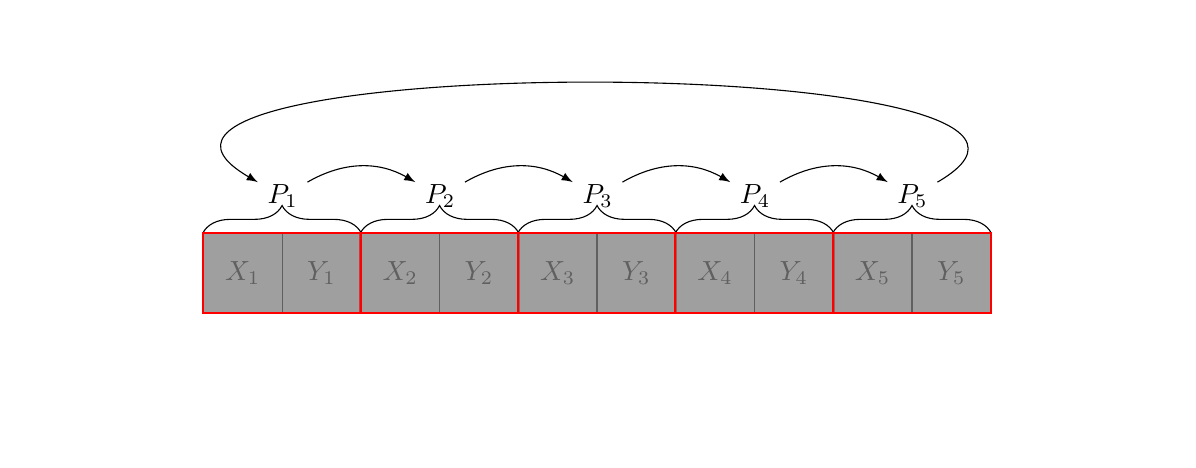
\begin{tikzpicture}
			\foreach \i in {1, ..., 5}{
				\node[draw=none] at (3, -2) {};
				\node[draw=none] at (3, 3) {};
				\node[rectangle, draw, minimum width=1cm, minimum height=1cm] (x\i) at (2*\i cm, 0) {$X_{\i}$};
				\node[rectangle, draw, minimum width=1cm, minimum height=1cm] (y\i) at (1cm + 2*\i cm, 0) {$Y_{\i}$};
				\draw<2->[decorate, decoration={brace, amplitude=10pt}] (x\i.north west) -- (y\i.north east);
				\node<2->[above=20pt of x\i.east] (p\i) {$P_{\i}$};
			}
			
			\foreach \i / \x in {1/2, 2/3, 3/4, 4/5, 5/1}{
				\draw<+ (2) ->[-latex] (p\i) to [out=30, in=150] ({p\x});
			}
			
			\foreach \i / \x in {1/2, 2/3, 3/4, 4/5}{
				\draw<+ (2)> [red, thick, fill=gray, fill opacity=.5] (x\i.north west) rectangle (y\x.south east);
			}
			\draw<+ (2)> [red, thick, fill=gray, fill opacity=.5] (x5.north west) rectangle (y5.south east);
			\draw<. (2)> [red, thick, fill=gray, fill opacity=.5] (x1.north west) rectangle (y1.south east);
		\end{tikzpicture}
	\end{figure}
\end{frame}

\begin{frame}{Oppgave 2c}
	\begin{figure}
		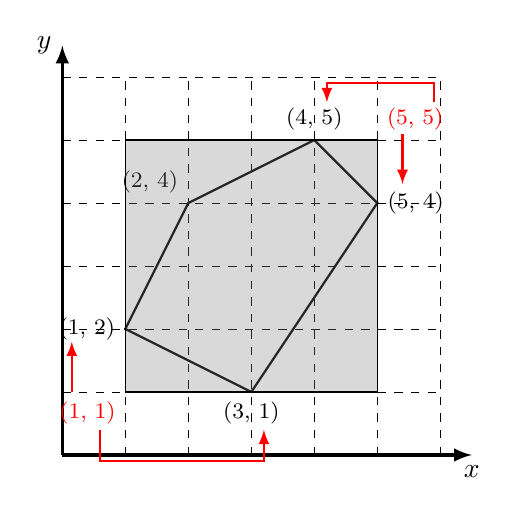
\begin{tikzpicture}[scale=.8]
			\draw<+->[dashed, very thin] (0, 0) grid (6, 6);
			\draw<.->[-latex, very thick] (0, 0) -- (6.5, 0) node[below] {$x$};
			\draw<.->[-latex, very thick] (0, 0) -- (0, 6.5) node[left] {$y$};
			
			\draw<.->[thick] (3, 1) -- (5, 4) node[right] (p1){\footnotesize(5, 4)}
				    -- (4, 5) node [above] (p2) {\footnotesize (4, 5)}
					-- (2, 4) node[above left] (p3) {\footnotesize (2, 4)}
					-- (1, 2) node[left] (p4) {\footnotesize (1, 2)}
					-- (3, 1) node[below] (p5) {\footnotesize (3, 1)};
			
			\draw<+->[fill=gray, fill opacity=.3] (1, 1) node[below left, fill opacity=1, color=red] {\footnotesize (1, 1)} rectangle (5, 5) node[above right, fill opacity=1, color=red] {\footnotesize (5, 5)};
			
			\draw<+->[-latex, color=red, thick] (0.15, 1) -- ++(0, .8);
			\draw<+->[-latex, color=red, thick] (0.6, 0.4) -- ++(0, -.5) -| (3.2, 0.4); 
			
			\draw<+->[-latex, color=red, thick] (5.4, 5.1) -- (5.4, 4.3);
			\draw<.->[-latex, color=red, thick] (5.9, 5.6) -- ++(0, 0.3) -| (4.2, 5.6);
			
		\end{tikzpicture}
	\end{figure}
\end{frame}

\begin{frame}{H2011 Oppgave 4}
	\begin{itemize}
		\item \href{https://www.ntnu.no/wiki/display/tdt4110/Python+eksamensoppgaver?preview=/78972128/79298929/Python2011.pdf}{På Wiki}
	\end{itemize}
\end{frame}

\begin{frame}{Oppgave 4c}
	\begin{figure}
		\newarray\names
		\readarray{names}{Albus&Fleur&Frank&Harry&Hermine&Minerva&Ron&Severus&Sirius&Vernon}%
		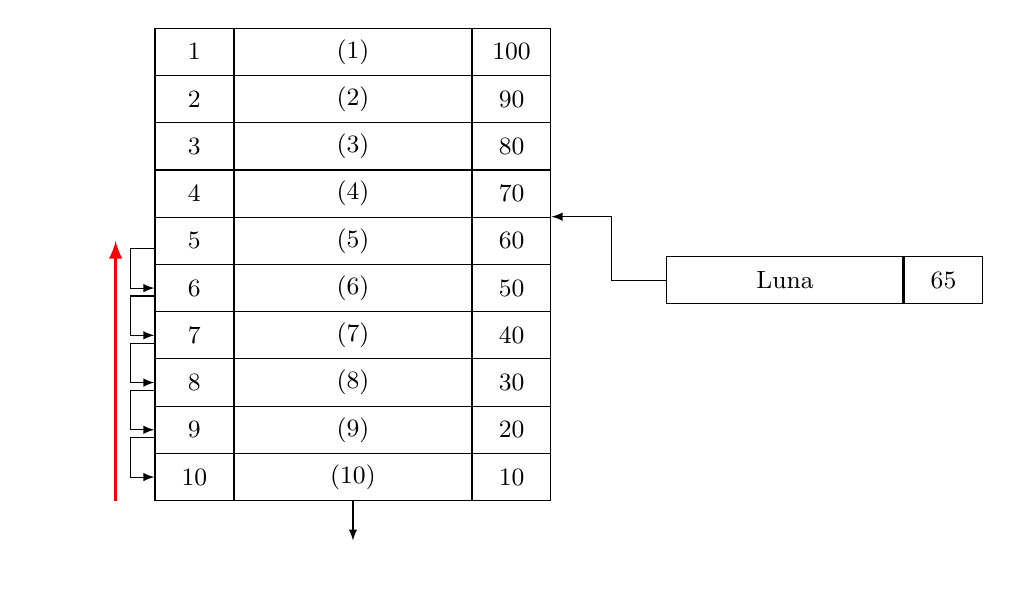
\begin{tikzpicture}[every node/.style = {font=\small}]
			\node[draw=none] at (-2cm, -7cm) {};
			
			\foreach[count=\i] \x in {100, 90, ..., 10}{
				\node<.->[rectangle, draw, minimum height=.6cm, minimum width=1cm] (num\i) at (0, -.6*\i cm) {\i};
				\node<.->[rectangle, draw, minimum height=.6cm, minimum width=3cm, right=0cm of num\i,] (name\i) {\names(\i)};
				\node<.->[rectangle, draw, minimum height=.6cm, minimum width=1cm, right=0cm of name\i] (score\i) {\x};
			}
			\node<+->[rectangle, draw, minimum height=.6cm, minimum width=3cm] (nameinsert) at (7.5cm, -3.5cm) {Luna};
			\node<.->[rectangle, draw, minimum height=.6cm, minimum width=1cm, right=0cm of nameinsert] (scoreinsert) {65};
			
			\draw<+-> [-latex] (nameinsert.west) -- ++(-.7cm, 0) |- (score5.north east);
			
			\foreach \i\x in {5/6, 6/7, 7/8, 8/9, 9/10} {
				\draw<+-> [-latex] ($(num\i.west) - (0, 1mm)$) -- ++ (-.3cm, 0) |- (num\x.west);
			}
			\draw<+->[-latex] (name10.south) -- ++(0, -.5cm);
			\draw<+->[-latex, red, very thick] (-1, -6.3) -- (-1, -3);
		\end{tikzpicture}
	\end{figure}
\end{frame}

\section{Spørsmål}

\begin{frame}{Takk for i år}
	\begin{itemize}
		\item Lykke til på eksamen
	\end{itemize}
\end{frame}

\end{document}
